\documentclass{article}
\usepackage[utf8]{inputenc}
\usepackage{graphicx}


\begin{document}


\begin{titlepage}
\begin{center}
{\Huge Cloud Application Project \par}
\vspace{18mm}
{\huge Alice Nannini \par}
{\huge Marco Parola \par}
{\huge Stefano Poleggi \par}
\vspace{18mm}
A.Y. 2019-2020
\end{center}

\end{titlepage}

% ----- INDICE -----
\tableofcontents\thispagestyle{empty}
\clearpage

\section{Introduction}
This cloud application is developed in order to manage, store and retrieve some data related to e-mails.\\
The model of an e-mail is the following:
\begin{verbatim}
    mail{
        id* : integer(\$int64),
        sender* : string,
        receiver* : string,
        mailText* : string
    }
\end{verbatim}
Using a web graphic interface it's possible interact with the application and execute the standard CRUD operations:
\begin{itemize}
\item \textbf{Create}: passing the field \textit{sender}, \textit{receiver} and \textit{mailText}, store a new e-mail.
\item \textbf{Read}: specifying an ID, retieve the information related to it.
\item \textbf{Update}: specifying an ID and passing the fields \textit{sender}, \textit{receiver} and \textit{mailText}, modify an existing e-mail.
\item \textbf{Delete}: specifying an ID, remove an e-mail from the system.
\end{itemize}
Please note that every commands you find are executed from the root directory stored in each vm.



\section{Architecture}
The following image shows the multi-tier architecture of the cloud application.
\begin{minipage}{\linewidth}
\begin{center}
\vspace{8mm}
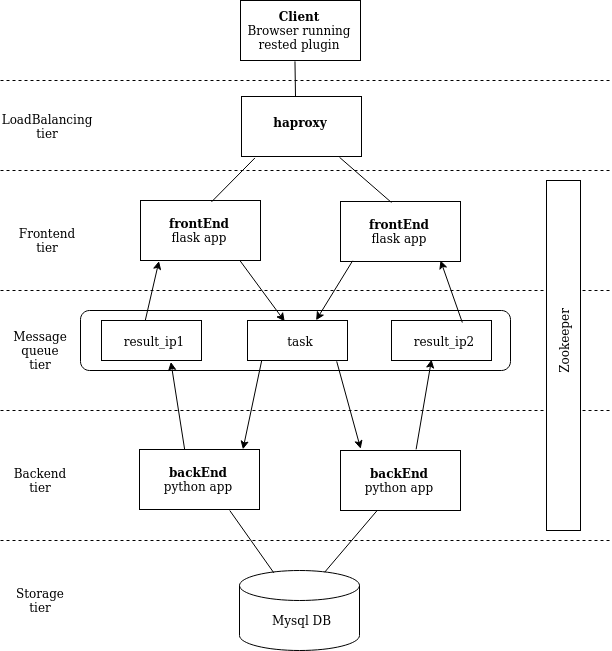
\includegraphics[height=11cm]{./img/architecture.png} 
\vspace{9mm}
\end{center}
\end{minipage}
Each module that composes the cloud application is run on a docker container.




\section{Client}
As client we use the Rested plugin available on all browsers, thanks to which we can perform the http request to interact with deeper layers.\\
\begin{minipage}{\linewidth}
\begin{center}
\vspace{8mm}
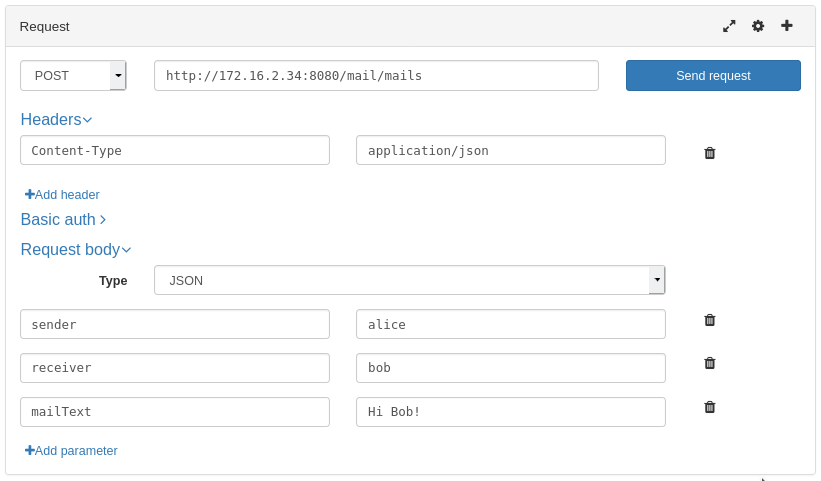
\includegraphics[height=7cm]{./img/rested.png} 
\vspace{8mm}
\end{center}
\end{minipage}
\section{Loadbalancing tier}
In order to evenly distribute the input traffic load among the two Front End servers of the application, a Load Balancer Tier is introduced. To implement that Tier we used HAProxy, which is a free and open-source solution for load balancing. \\
After downloading the docker image, we configure the proxy to make it able to sort the requests on our two servers. Following we have the haproxy.cfg file, with all the configuration setted for our application
\begin{verbatim}
    backend myAppBackEnd
        balance roundrobin
        mode http
        server myAppServer1 172.16.1.249:8080 check
        server myAppServer2 172.16.2.57:8080 check
\end{verbatim}
\vspace{3mm}
In particular, the last block (MyAppBackend) is the one in which we configured our frontend dispatching process. 
\begin{itemize}
\item roundrobin: load balancing algorithm
\item myAppServer1, myAppServer2: the name of the servers to which we dispatch the requests
\item 172.16.1.249, 172.16.2.57: ip addresses of the servers
\item 8080: port on which the servers listen for requests
\item check: specifies to check the health of the servers
\end{itemize}
\subsection{Commands}  
\begin{verbatim}
    docker build -t ha loadBalancer/
    docker run -d -p 8080:80 -p 9999:9999 --name haproxy ha
\end{verbatim}




\section{Frontend}
The Frontend has been developed starting from the SWAGGER tool, which allowed us to build up a Python Flask server. We modified that Flask Server in order to suit it to our application.\\
All parameters useful for connection between Frontend and RabbitMQ Server, our message broker, are retrieved using the Zookeeper service; once the connection among these two tier has been established, the Frontend is ready to publish all requests to the “task” queue and wait for the response that will be placed by the Backend instance. 
\subsection{Commands}
\begin{verbatim}
    docker build -t fe frontEnd/
    docker run -p 8080:8080 --name myfe fe
\end{verbatim}




\section{Message queue system}
In order to introduce a time and space decoupling, we implemented a message queue system using a RabbitMQ Server. That tier has been realized using the rabbitmq:3 image.\\
The message queuing system handles only direct exchanges; there are 5 queues, the “task” queue is the one in which the Frontend instances place all their requests, while Backend instances performs the operations specified in the tasks and places the response in the correct queue. In particular, there are 4 response queue, one for each possible operation (create, read, update and delete). \\
Finally, to make the server reachable remotely, a new user (\textit{root}) with all the possible credentials has been created and registered to the server.
\subsection{Commands}
\begin{verbatim}
    docker build -t mb broker/
    docker run -d -p 5672:5672 --name mymb mb
    docker exec mymb rabbitmqctl add_user root root
    docker exec mymb rabbitmqctl set_user_tags root administrator
    docker exec mymb rabbitmqctl set_permissions -p / root ".*" ".*" ".*"
\end{verbatim}




\section{Backend tier}
Backend instances interact directly with the storage tier and perform requests coming from Frontend, retrieving those requests from the “task” queue. Once retrieved a request, the backends execute the operation requested via a specific query. Once the operation is completed, those instances prepare a response (which is already in a response code, data format) and place it in the specific queue.\\
Once again, all parameters for MySQL and RabbitMQ are retrieved via the Zookeeper service.
\subsection{Commands}
\begin{verbatim}
    docker build -t be backEnd/
    docker run -d --name mybe be
\end{verbatim}




\section{Storage tier}
To realize the storage tier, we used a MySQL docker container. After exploiting the docker, we created the table 'mails' needed to store our data.
\begin{minipage}{\linewidth}
\begin{center}
\vspace{8mm}
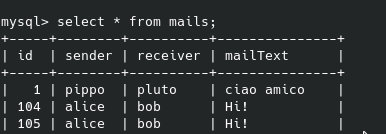
\includegraphics[height=2.5cm]{./img/mysql.png} 
\vspace{3mm}
\end{center}
\end{minipage}
\subsection{Commands}
\begin{verbatim}
    docker pull mysql/mysql-server:latest
    docker run --name=mydb -d -p 3306:3306 mysql/mysql-server:latest
    apt-get install mysql-client
    docker exec -it mydb mysql -uroot -p


    >> ALTER USER 'root'@'localhost' IDENTIFIED BY 'newpassword';
    >> use mysql;
    >> UPDATE user SET host='%' WHERE host='localhost' AND user='root';
    >> FLUSH PRIVILEGES;


    >> CREATE SCHEMA `mails`;
    >> CREATE TABLE `mails`.`mails` (
    >>     `id` INT(11) NOT NULL AUTO_INCREMENT,
    >>     `sender` VARCHAR(50) NOT NULL,
    >>     `receiver` VARCHAR(50) NOT NULL,
    >>     `mailText` TEXT NOT NULL,
    >>     PRIMARY KEY (`id`)
    >> ) ENGINE=InnoDB DEFAULT CHARSET=utf8mb4 ;


    >> exit
\end{verbatim}



\section{Zookeeper}
Moreover there is an additional layer: Zookeeper. It is a service for distributed systems, used for data exchange among different services of an application. For that reason, we used it to provide configuration parameters to frontend and backend instances. Particularly we provided:
\begin{itemize}
\item RabbitMQ’s server address, port, username and password to frontend and backend.
\item MySQL’ s server address, username, password and database name to backend.
\end{itemize}
\subsection{Commands}
We executed the following commands in each node running frontend or back layer.
\begin{verbatim}
    docker run -d 
   -p 2181:2181 
   -p 2888:2888 
   -p 3888:3888 
   --name myzk-1 
   -e ZOO_MY_ID=1 
   -e ZOO_SERVERS='server.1=<ip_1>:2888:3888;2181 
                server.2=<ip_2>:2888:3888;2181 
                server.3=<ip_3>:2888:3888;2181' 
    --restart always 
    zookeeper
\end{verbatim}
From the python shell of one vm we ran the following python code to setup the shared values. We exploited the \textit{kazoo} library.
\begin{verbatim}
    from kazoo.client import KazooClient

    hosts = "172.16.3.50:2181,172.16.1.249:2181,172.16.2.57:2181"

    zk = KazooClient(hosts=hosts, read_only=True)
    zk.start()

    path = "/myApp"

    #Store the data
    if zk.exists(path):
        zk.delete(path, recursive=True)

    zk.ensure_path(path)
    zk.create(path+"/broker_addr", b"172.16.2.57") 
    zk.create(path+"/broker_port", b"5672")
    zk.create(path+"/broker_user", b"root")
    zk.create(path+"/broker_psw", b"root")
    zk.create(path+"/db_addr", b"172.16.2.57")
    zk.create(path+"/db_user", b"root")
    zk.create(path+"/db_psw", b"newpassword")
    zk.create(path+"/db_name", b"mails")

    exit(0)
\end{verbatim}
\end{document}


